
% This work is licensed under the Creative Commons Attribution-Share Alike 2.0 France License.
% To view a copy of this license, visit http://creativecommons.org/licenses/by-sa/2.0/fr/legalcode
% or send a letter to Creative Commons, 171 Second Street, Suite 300, San Francisco, California, 94105, USA.

\chapter{Réponses aux «~À vous de jouer~»\label{annexe:reponses}}


Vous trouverez ici les réponses aux questions posées dans la plupart des chapitres dans la section «~À vous de jouer~». 

\section{Réponses aux cas pratiques de la section \ref{PRATIQUE:8}\label{REPONSES:8}}
\begin{enumerate}
\item La réponse à l'\textbf{exercice 1} devrait ressembler à ce qui suit:\\

\begin{small}
\begin{Verbatim}[frame=single,rulecolor=\color{mbleu}, label=à taper]
>>> jouets= [ 'Lego', 'Playmo', 'mandala', 'vélo' ]
>>> plats = [ 'crêpes', 'gaufres', 'betterave' ]
>>> préférés = jouets + plats
>>> print(préférés)
['Lego', 'Playmo', 'mandala', 'vélo', 'crêpes', 'gaufres', 'betterave']
\end{Verbatim}
%\rm
\end{small}
\item  La réponse à l'\textbf{exercice 2} est simplement d'ajouter le résultat de «~\texttt{3*25}~» et le résultat de «~\texttt{10*32}~». L'équation suivant montre le résultat de cette équation:

\begin{Verbatim}[frame=single,rulecolor=\color{mbleu}, label=à taper]
>>> print(3 * 25 + 10 * 32)
395
\end{Verbatim}
\rm
\emph{Ce qui fait beaucoup de friandises!}\\

Néanmoins, si vous avez suivi la partie sur l'usage de parenthèses dans le chapitre \ref{chap:8}, vous pouvez avoir décidé de mettre des parenthèses dans cette équation. Vous devriez avoir fait quelque chose comme:
\tt
\begin{Verbatim}[frame=single,rulecolor=\color{mbleu}, label=à taper]
>>> print((3 * 25) + (10 * 32))
395
\end{Verbatim}
\rm

La réponse est la même, car la multiplication est faite avant l'addition. Dans les deux équations les deux multiplications sont faites en premier et les résultats sont additionnés. Malgré tout la seconde équation est peut-être légèrement meilleure que la première. En effet, l'ordre des opérations est immédiatement évident pour le lecteur. Un programmeur moins compétent (qui ne connaîtrait pas aussi bien l'ordre des opérations) pourrait penser que dans la première équation vous multipliez 3 par 25, puis additionnez 10 et multipliez le résultat par 32 (la réponse complément fausse est 2720). Avec les parenthèses, il est un peu plus simple de comprendre ce qui est calculé en premier.

\item  La réponse à l'\textbf{exercice 2} devrait ressembler à:
\tt
\begin{Verbatim}[frame=single,rulecolor=\color{mbleu}, label=à taper]
>>> prénom = 'Morgane'
>>> nom = 'Paul'
>>> print('Mon nom est %s %s.' % (prénom, nom))
Mon nom est Morgane Paul.
\end{Verbatim}
\rm

\end{enumerate}

\section{Réponses aux cas pratiques de la section  \ref{PRATIQUE:TORTUES}\label{REPONSES:TORTUES}}
\begin{enumerate}
\item La réponse à l'\textbf{exercice 1} devrait ressembler à ce qui suit: un rectangle est semblable à un carré mis à part que deux côtés peuvent être plus longs que les deux autres. En disant à la tortue de faire les actions suivantes, vous pouvez aisément dessiner un rectangle:
\begin{itemize}
 \item avancer d'un certain nombre de points;
 \item tourner à angle droit;
 \item avancer d'un certain nombre de points;
 \item tourner à angle droit dans le même sens que la première rotation;
 \item avancer du même nombre de points que pour le premier déplacement;
 \item tourner à angle droit dans le même sens que la première rotation;
 \item avancer du même nombre de points que pour le deuxième déplacement.
\end{itemize}

Par exemple, le code suivant tracera un rectangle que vous pouvez voir sur la \autoref{fig46}.
\begin{Verbatim}[frame=single,rulecolor=\color{mbleu}, label=à taper]
import turtle

tortue = turtle.Pen()
tortue.forward(150)
tortue.left(90)
tortue.forward(50)
tortue.left(90)
tortue.forward(150)
tortue.left(90)
tortue.forward(50)
\end{Verbatim}


\begin{figure}[!ht]
\begin{center}
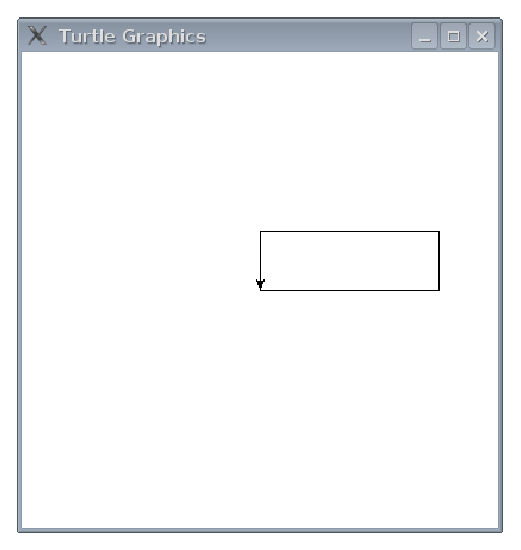
\includegraphics[width=82mm]{images/rectangletortue.eps}
\end{center}
\caption{Tortue dessinant un rectangle.}\label{fig46}
\end{figure}

\item La réponse à l'\textbf{exercice 2} devrait ressembler à ce qui suit:

Un triangle est un peu plus compliqué à dessiner car vous avez besoin de connaître plus d'informations sur les angles et les longueurs des côtés. Si vous n'avez pas étudié les angles à l'école cela pourrait être un peu plus difficile que vous ne vous y attendiez. Vous pouvez dessiner un triangle simple (voir la \autoref{fig:trianglesimple} avec le code suivant:

\begin{Verbatim}[frame=single,rulecolor=\color{mbleu}, label=à taper]
import turtle

tortue = turtle.Pen()
tortue.forward(100)
tortue.left(135)
tortue.forward(70)
tortue.left(90)
tortue.forward(70)
\end{Verbatim}

\begin{figure}[!ht]
\begin{center}
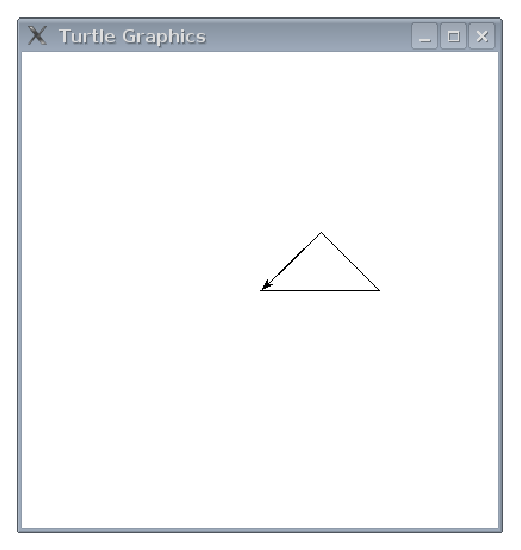
\includegraphics[width=82mm]{images/trianglesimple.eps}
\end{center}
\caption{La tortue dessine un triangle}\label{fig:trianglesimple}
\end{figure}

\end{enumerate}

\section{Réponses aux cas pratiques de la section  \ref{PRATIQUE:BOUCLES}\label{REPONSES:BOUCLES}}
\begin{enumerate}
\item La réponse à l'\textbf{exercice 1} est que seule la chaîne \texttt{x vaut 0} sera affichée. Regardons le code en détail pour comprendre pourquoi.
\begin{Verbatim}[frame=single,rulecolor=\color{gray}, label=ne pas taper]
>>> for x in range(0, 20):
... 	print('x vaut %s' % x)
... 	if x < 9:
... 		break
x vaut 0
\end{Verbatim}

La raison en est que durant la première itération la valeur de variable \texttt{x} est zéro. Comme zéro vaut moins que neuf, la commande \texttt{break} est lancée et fait sortir de la boucle.

\item Pour répondre à l'\textbf{exercice 2} je vous propose d'écrire un petit programme qui va calculer le nombre de nénuphars chaque jour et l'afficher. Quand le nombre de nénuphars dépassera mille il suffit d'arrêter la boucle.

Pour information voila à quoi peut ressembler un tel programme.
\begin{Verbatim}[frame=single,rulecolor=\color{gray}, label=ne pas taper]
>>> jours = 0
>>> nénuphars = 1
>>> while nénuphars < 1000:
...     jours+=1
...     nénuphars*=2 
...     print('Au bout de %s jours, il y a %s nénuphars.' 
...            % (jours, nénuphars))
... 
Au bout de 1 jours, il y a 2 nénuphars.
Au bout de 2 jours, il y a 4 nénuphars.
Au bout de 3 jours, il y a 8 nénuphars.
Au bout de 4 jours, il y a 16 nénuphars.
Au bout de 5 jours, il y a 32 nénuphars.
Au bout de 6 jours, il y a 64 nénuphars.
Au bout de 7 jours, il y a 128 nénuphars.
Au bout de 8 jours, il y a 256 nénuphars.
Au bout de 9 jours, il y a 512 nénuphars.
Au bout de 10 jours, il y a 1024 nénuphars.
>>> print("Il faut seulement %s jours pour 
...que le lac soit envahi." % jours)
Il faut seulement 10 jours pour que le lac soit envahi.
\end{Verbatim}

Aux deux premières lignes nous initialisons les variables «~\verb+nénuphars+~» à un et «~\verb+jours+~» à zéro.  
À la troisième ligne nous créons une boucle «~tant que~» en utilisant comme condition d'arrêt que le nombre de nénuphars devient supérieur ou égal à mille. Puis, dans le bloc nous augmentons le nombre de jours de un jour à chaque pas et multiplions le nombre de nénuphars par deux à chaque pas. Enfin, nous affichons le résultat du calcul de chaque pas. Une fois sortis de la boucle nous synthétisons le résultat. 
\end{enumerate}

\section{Réponses aux cas pratiques de la section  \ref{PRATIQUE:RECYCLAGE}\label{REPONSES:RECYCLAGE}}
\begin{enumerate}
\item La réponse à l'\textbf{exercice 1} devrait ressembler à ce qui suit: 

Transformer la boucle tant que en fonction est vraiment très simple. Votre fonction devrait ressembler à ça.

\begin{Verbatim}[frame=single,rulecolor=\color{mbleu}, label=à taper]
>>> def calcul_nénuphars(nénuphars,coefficient):
...     jours=0
...     while  nénuphars < 1000:
...         jours+=1
...         nénuphars*=coefficient
...         print('Au bout de %s jours, il y a %s nénuphars.' % 
...(jours, nénuphars))
...     print("Avec un coefficient de %s, Il faut %s 
...jours pour que le lac soit envahi" % (coefficient,jours))
\end{Verbatim}

Si vous comparez la fonction avec le code initial, vous devriez remarque que, sauf pour la première ligne, le code n'a presque pas changé. Seul le «~\texttt{*=2}~» a été changé en «~\texttt{*=coefficient}~». La dernière dernière ligne a, elle aussi, était modifiée mais uniquement pour changer l'information affichée. Comme «~\texttt{nénuphars}~» était déjà une variable, il n'y a pas de changement à faire quand nous l'utilisons comme un paramètre. Vous pouvez contrôler que le résultat est le même quand vous utilisez le code dans une fonction ou en dehors\footnote{Une bonne habitude de de créer le maximum de fonction, ce n'est pas compliqué à faire et on ne sait jamais: cela pourra toujours être utilisé ailleurs.}.

\begin{Verbatim}[frame=single,rulecolor=\color{mbleu}, label=à taper]
>>> calcul_nénuphars(1, 2)
Au bout de 1 jours, il y a 2 nénuphars.
Au bout de 2 jours, il y a 4 nénuphars.
Au bout de 3 jours, il y a 8 nénuphars.
Au bout de 4 jours, il y a 16 nénuphars.
Au bout de 5 jours, il y a 32 nénuphars.
Au bout de 6 jours, il y a 64 nénuphars.
Au bout de 7 jours, il y a 128 nénuphars.
Au bout de 8 jours, il y a 256 nénuphars.
Au bout de 9 jours, il y a 512 nénuphars.
Au bout de 10 jours, il y a 1024 nénuphars.
Avec un coefficient de 2, Il faut 10 jours pour que le lac soit 
envahi.
\end{Verbatim}

\item La réponse à l'\textbf{exercice 2} devrait ressembler à ce qui suit: 
\begin{Verbatim}[frame=single,rulecolor=\color{mbleu}, label=à taper]
>>> def calcul_nénuphars(nénuphars,coefficient,jours_max):
...     jours=0
...     while  jours < jours_max:
...         jours+=1
...         nénuphars*=coefficient
...     print('''Au bout de %s jours avec un coefficient de %s, 
...il y a %s nénuphars.''' % ...(jours, coefficient, nénuphars))
\end{Verbatim}
Changer la fonction pour passer le nombre de jours comme un paramètre n'a demandé qu'un faible nombre de changements.

Nous pouvons maintenant facilement changer le nombre de nénuphars, le coefficient de croissance et le nombre de jours:

\begin{Verbatim}[frame=single,rulecolor=\color{mbleu}, label=à taper]
>>> calcul_nénuphars(2, 1.5, 20)
Au bout de 20 jours avec un coefficient de 1.5, 
il y a 6650.51346016 nénuphars.
\end{Verbatim}
Nous remarquons que notre programme permet d'avoir des bouts de nénuphars, en effet le nombre de nénuphars est un nombre à virgule. Nous imaginerons que les bouts de nénuphars sont des bébés ou des petits nénuphars. Python pourrait gérer ce genre de problème mais ce n'est pas l'objet de ce livre.

\item La réponse à l'\textbf{exercice 3} devrait ressembler à ce qui suit: 
Si vous avez gardé la session python ouverte vous n'avez pas à redéfinir la fonction «~\texttt{calcul\_nénuphars}~». De plus les questions affichées sont aussi optionnelles, vous apprendrez dans le chapitre suivant à sauvegarder vos programmes et l'affichage des questions deviendra alors importante car elle seront posées à des tiers (d'autres personnes).

\begin{Verbatim}[frame=single,rulecolor=\color{mbleu}, label=à taper]
>>> def calcul_nénuphars(nénuphars,coefficient,jours_max):
...     jours=0
...     while  jours < jours_max:
...         jours+=1
...         nénuphars*=coefficient
...     print('Au bout de %s jours avec un coefficient de %s, 
...il y a %s nénuphars.' % ...(jours, coefficient, nénuphars))
>>> import sys
>>> def demande() : 
>>>     print('Entrez le nombre initial de nénuphars :')
>>>     rnénuphars = float(sys.stdin.readline())
>>>     print('Entrez le nombre de coefficient :')
>>>     rcoefficient = float(sys.stdin.readline())
>>>     print('Entrez le nombre de jours :')
>>>     rjours = float(sys.stdin.readline())
>>>     calcul_nénuphars(rnénuphars, rcoefficient, rjours)
>>> demande()
Entrez le nombre initial de nénuphars :
2
Entrez le nombre de coefficient :
1.2
Entrez le nombre de jours :
3
Au bout de 5 jours avec un coefficient de 1.2, il y a 4.97664 nénuphars.\end{Verbatim}
\end{enumerate}

\section{Réponses aux cas pratiques de la section  \ref{PRATIQUE:PROFUSION}\label{REPONSES:PROFUSION}}
\begin{enumerate}
\item Pour répondre à la première question il y a la manière facile et la manière difficile. La manière difficile n'est pas difficile car elle est compliquée. Elle est difficile car elle demande de taper beaucoup de choses:
\begin{Verbatim}[frame=single,rulecolor=\color{gray}, label=na pas saisir]
import turtle
tortue = turtle.Pen()
tortue.forward(50)
tortue.right(45)
tortue.forward(50)
tortue.right(45)
tortue.forward(50)
tortue.right(45)
tortue.forward(50)
tortue.right(45)
tortue.forward(50)
tortue.right(45)
tortue.forward(50)
tortue.right(45)
tortue.forward(50)
tortue.right(45)
tortue.forward(50)
\end{Verbatim}

Vous pouvez voir dans ce code que nous disons à la tortue d'avancer de cinquante pixels puis de tourner à droite de quarante-cinq degrés. Nous le faisons huit fois! Ce qui fait sept fois de trop. La manière la plus simple est présentée ci-dessous, elle produit aussi l'octogone que vous pouvez observer sur la \autoref{fig:octogone}.
\begin{Verbatim}[frame=single,rulecolor=\color{mbleu}, label=à taper]
import turtle
tortue = turtle.Pen()
for x in range(0,8):
    tortue.forward(50)
    tortue.right(45)
\end{Verbatim}

\begin{figure}
\begin{center}
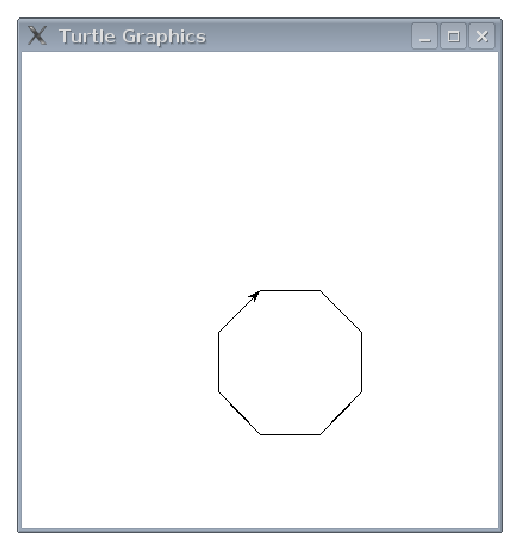
\includegraphics[width=82mm]{images/octogone.eps}
\end{center}
\caption{La tortue dessine un octogone.}\label{fig:octogone}
\end{figure}

\item Si vous regardez à nouveau les fonctions étudiées dans \autoref{chap:tortue2}, vous verrez comme créer une forme remplie. Nous pouvons convertir notre code de dessin d'un octogone en une fonction qui utilise une couleur et nous voulons aussi pouvoir réutiliser cette fonction par la suite.

\begin{Verbatim}[frame=single,rulecolor=\color{mbleu}, label=à taper]
import turtle
tortue = turtle.Pen()
def octogone(red, green, blue):
    tortue.color(red, green, blue)
    tortue.begin_fill()
    for x in range(0,8):
        tortue.forward(50)
        tortue.right(45)
    tortue.end_fill()
octogone(0, 0, 1)
\end{Verbatim}

Nous fixons une couleur puis démarrons le remplissage. Puis nous lançons la boule pour dessiner un octogone, puis nous arrêtons le remplissage pour que Python remplisse la forme que nous venons de dessiner. 


\begin{figure}
\begin{center}
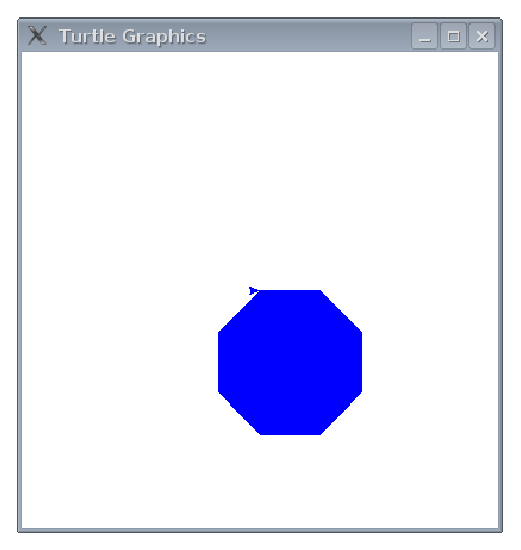
\includegraphics[width=82mm]{images/octogonebleu.eps}
\end{center}
\caption{La tortue dessine un octogone bleu.}\label{fig:octogonebleu}
\end{figure}
\end{enumerate}